In 1915, Albert Einstein published his theory of general relativity, a 
geometric theory of gravitation that sought to expand upon Newtonian 
mechanics and provide a complete description of gravity and its 
relationship with space and time. Einstein theorized that space 
and time were deeply related and existed together as a manifold 
called spacetime. Matter with energy and momentum 
existing in this manifold would create 
curvature in spacetime. Gravitational forces were the result of 
matter following geodesic curves in spacetime. This concept can 
be summarized in the Einstein field equation, which is presented 
as,
\begin{equation}
G_{\mu\nu} = 8\pi T_{\mu\nu}
\label{eq:EFE}
\end{equation}
where $G_{\mu\nu}$ is the Einstein tensor, which describes the 
curvature of spacetime, $T_{\mu\nu}$ is the 
stres-energy tensor, which describes the energy and momentum in 
spacetime, and  $G=c=1$. The Einstein tensor is defined as,
\begin{equation}
G_{\mu\nu} = R_{\mu\nu} - \frac{1}{2}Rg_{\mu\nu}
\end{equation}
where $R_{\mu\nu}$ is the Ricci curvature tensor and $g_{\mu\nu}$ is 
the metric tensor for the manifold.

An interesting result that arises from this formalism is the 
existence of gravitational waves, which are perturbations in 
spacetime caused by certain types of time-varying mass distributions. 
To describe gravitational waves, we consider 
a Minkowski metric with a small perturbation. The Minkowski metric 
is a flat spacetime metric defined as
\begin{equation}
\eta_{\mu\nu} = 
  \begin{pmatrix}
   -1 & 0 & 0 & 0 \\
    0 & 1 & 0 & 0 \\
    0 & 0 & 1 & 0 \\
    0 & 0 & 0 & 1
  \end{pmatrix}
\end{equation}
where $\mu = 0$ corresponds to the time coordinate and $\mu = {1,2,3}$ 
correspond to the spatial coordinates. In examples, we will use the coordinate 
convention $(x^0,x^1,x^2,x^3) = (ct,x,y,z)$. 
The full spacetime metric, $g_{\mu\nu}$, is then constructed as a 
linear perturbation on the Minkowski metric,
\begin{equation}
g_{\mu\nu} = \eta_{\mu\nu} + h_{\mu\nu}
\end{equation}
where $h_{\mu\nu}$ is the metric perturbation and $|h_{\mu\nu}| \ll 1$.
From here, we follow the convention of Saulson \cite{Saulson:1994} to arrive at the general 
form of a gravitational wave.
At this point it is very useful to move into the transverse traceless 
gauge where coordinates on the manifold are defined by the geodesic 
motion of freely-falling test masses. In this gauge, the weak field 
vacuum solution of the Einstein field equation becomes a wave equation: 
\begin{equation}
\square h_{\mu\nu} = 0.
\end{equation}
The solutions to this differential equation will be plane waves of 
the form
\begin{equation}
h_{\mu\nu} = C_{\mu\nu}e^{i(2\pi ft - \vec{k}\cdot\vec{x})}
\end{equation}
where $C_{\mu\nu}$ is the wave amplitude, $f$ is the frequency, 
and $\vec{k}$ is the wave vector which indicates the direction of 
propagation \cite{Carroll}.

For example, consider the case of a gravitational 
wave propogating along the $\hat{z}$-axis.
When the conditions of the transverse traceless gauge are applied, 
the resulting form of $h_{\mu\nu}$ is 
\begin{equation}
h_{\mu\nu} = 
  \begin{pmatrix}
    0 & 0 & 0 & 0 \\
    0 & h_+ & h_x & 0 \\
    0 & h_x & -h_+ & 0 \\
    0 & 0 & 0 & 0
  \end{pmatrix}
\end{equation}
where the diagonal and off-diagonal terms represent two polarizations 
of the resulting gravitational wave, called "h-plus" and "h-cross" 
respectively.
We can see the effects of this perturbation by observing the  
spacetime interval on the manifold. The spacetime interval is defined as 
\begin{equation}
ds^2 = dx^\mu g_{\mu\nu}dx^\nu.
\end{equation}
Substituting in our perturbed metric for $g_{\mu\nu}$, we find that 
the spacetime interval can be broken up into a standard Minkowski line 
element and a perturbation due to $h_{\mu\nu}$.
\begin{equation}
ds^2 = dx^\mu (\eta_{\mu\nu} + h_{\mu\nu})dx^\nu \\
\end{equation}
\begin{equation}
ds^2 = dx^\mu \eta_{\mu\nu} dx^\nu + dx^\mu h_{\mu\nu}dx^\nu
\label{eq:spacetime}
\end{equation}

As an example, we present the case of a plus-polarized gravitational wave 
propagating in the $\hat{z}$ direction and observe the effect of the perturbation 
on the spacetime interval. The perturbation will have the form 
\begin{equation}
h_{\mu\nu} = 
  \begin{pmatrix}
    0 & 0 & 0 & 0 \\
    0 & h_+ & 0 & 0 \\
    0 & 0 & -h_+ & 0 \\
    0 & 0 & 0 & 0
  \end{pmatrix}
\end{equation}
Using the coordinate convention of $(ct,x,y,z)$, the unperturbed
spacetime interval is given as: 
\begin{equation}
ds^2 = -c^2 dt^2 + dx^2 + dy^2 + dz^2.
\end{equation}
Since the perturbation is spatially transverse to the direction of 
propagation, the ct- and z-coordinates will not be modulated by the 
gravitational wave. The x- and y-coordinates will be modulated  
according to equation \ref{eq:spacetime}. The resulting spacetime 
interval is
\begin{equation}
ds^2 = -c^2 dt^2 + (1 + h_+)dx^2 + (1 - h_+)dy^2 + dz^2.
\end{equation}
This shows that a gravitational wave propogating along the $\hat{z}$-axis 
will differentially stretch and squeeze spacetime in the transverse 
axes. The exact form of $h_+$ will depend on the source of the 
gravitational waves. A visualization of this stretching and squeezing 
is shown in Figure \ref{fig:polarizations}\cite{Polarization}. The cross polarization  
stretches and squeezes at a 45 degree angle relative to the plus 
polarization. The strain, $h_+$, imparted by a gravitational wave is 
typically extremely small by the time it reaches Earth, producing 
differential length changes on the order of $10^{-18}$m. 

\begin{figure}[ht!]
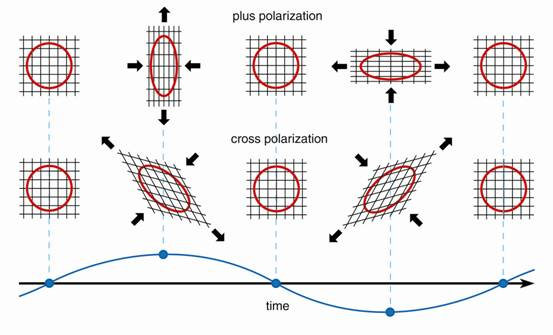
\includegraphics[width=\textwidth]{figures/introduction/polarisations2}
\caption[Plus and cross polarizations]{Plus and cross polarizations %
         of a gravitational wave.}
\label{fig:polarizations}
\end{figure}

The Advanced LIGO interferometers are designed to be sensitive 
to this differential stretching and squeezing by constructing orthogonal 
optical cavities. A gravitational wave passing through an aLIGO interferometer 
will differentially 
modulate the lengths of the optical cavities, creating an interference 
pattern at the output of the instrument that can be searched for 
gravitational wave signals. The layout and gravitational wave readout scheme 
of the interferometers is discussed below.

\section{The Advanced LIGO Interferometers}\label{sec:aligo}

The Advanced LIGO (aLIGO) interferometers are a pair of dual-recycled Michelson interferometers 
that employ 4km long Fabry-Perot cavities in their arms to increase the interaction time with a 
gravitational wave signal. 
Figure \ref{fig:aligo} shows a simplified layout of an aLIGO interferometer. 

\begin{figure}[ht!]
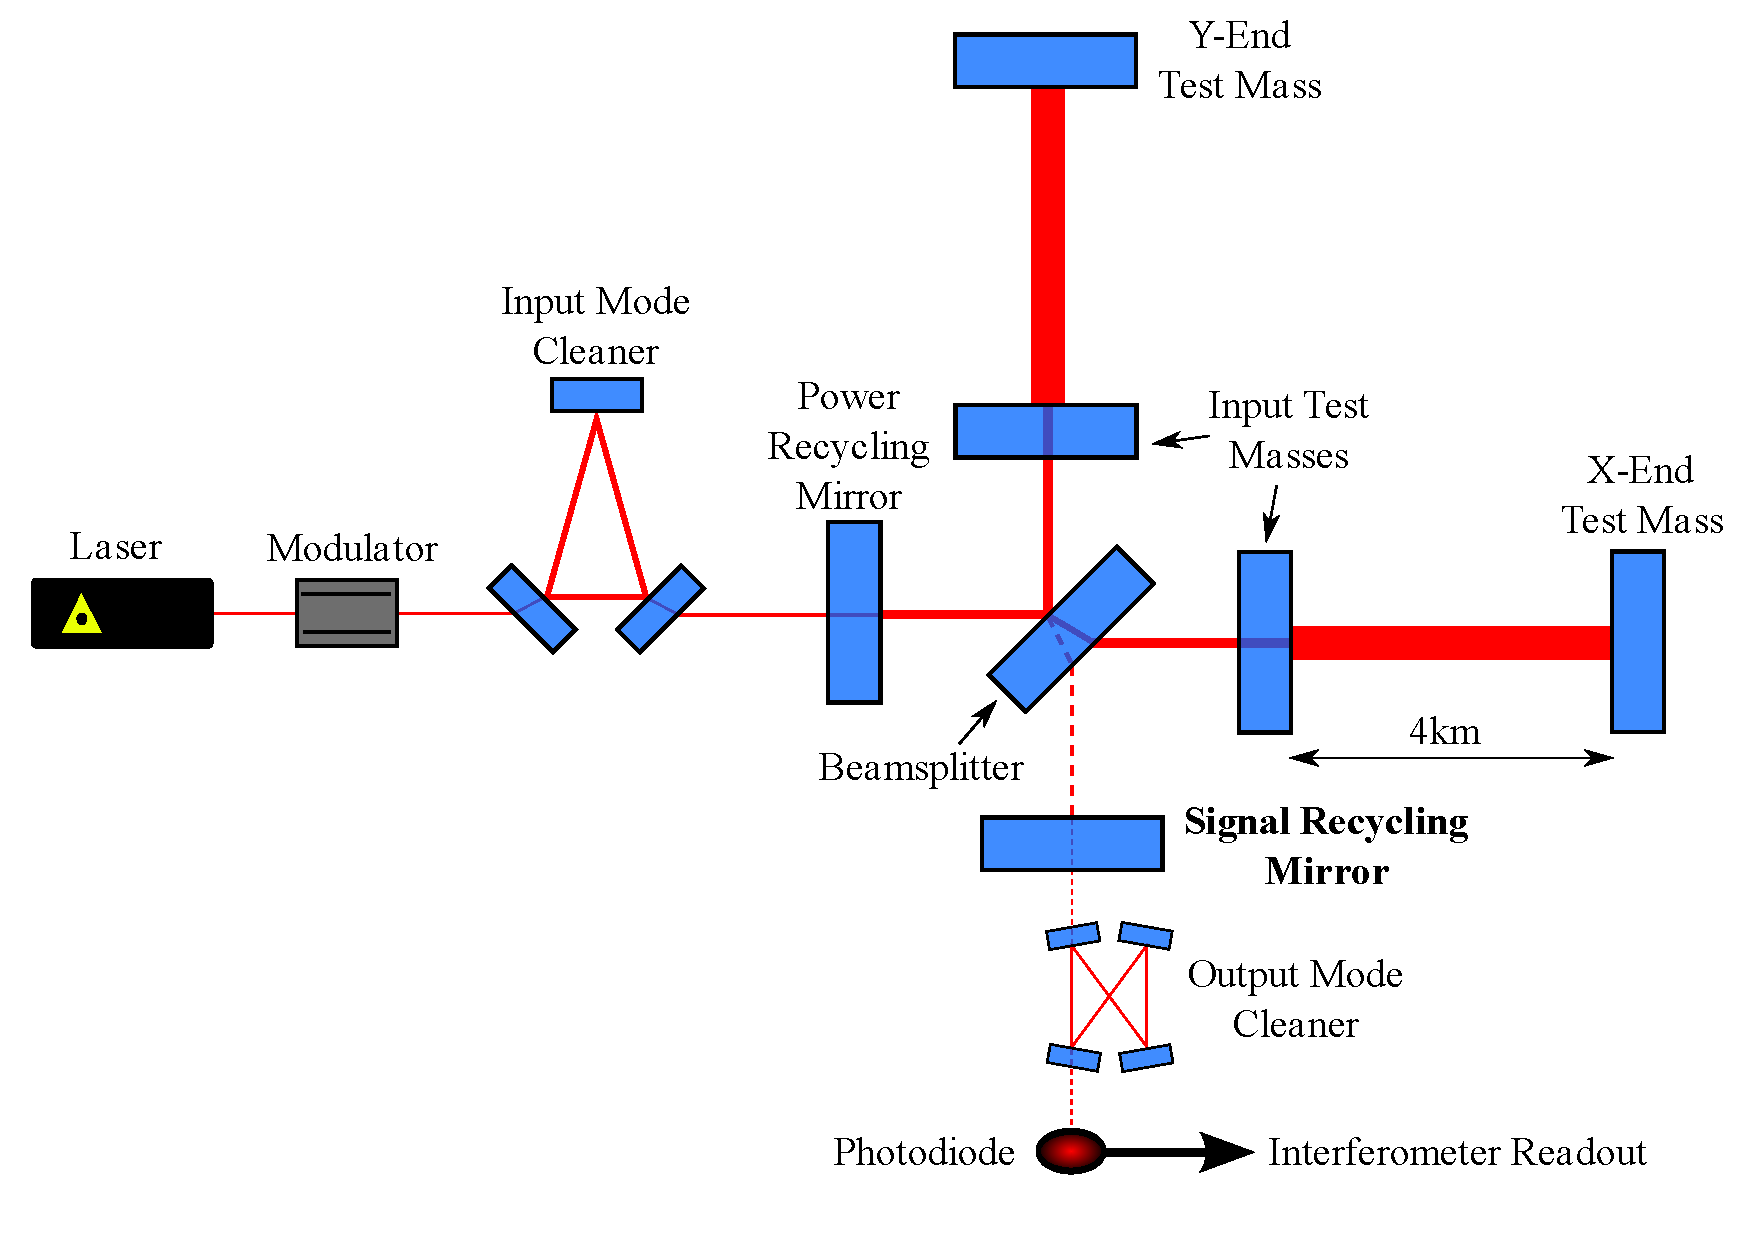
\includegraphics[width=\textwidth]{figures/introduction/ALIGO_layout}
\caption[Layout of Advanced LIGO]{Layout of Advanced LIGO}
\label{fig:aligo}
\end{figure}

At the input to an aLIGO interferometer is a solid-state Nd:YAG laser that provides laser light 
at a wavelength of 1064 nm. Not included in Figure \ref{fig:aligo} are frequency and 
intensity stabilization control loops designed to provide as stable a laser source as 
possible for the experiment. This stabilized laser is called the pre-stabilized laser 
(PSL). The laser light is passed through a series of 
electro-optic modulators (EOM) where radio-frequency (RF) sidebands are generated 
and imparted onto the light. These RF sidebands are used to control auxiliary optical 
degrees of freedom in the interferometer. The beam is then passed through the 
input mode cleaner (IMC), which rejects higher order spatial modes of the beam 
and transmits a circular TEM00 mode to be used in the instrument.

Once the beam has been stabilized in frequency and intensity and the higher order 
optical modes have been stripped away, it is transmitted through the power 
recycling mirror and enters the vertex of the interferometer. In the vertex, 
the beam is split 50/50 by the beamsplitter. Half of the light is directed toward  
the input test mass (ITM) of the X-arm and half of the light is directed  
toward the ITM of the Y-arm. As mentioned previously, the aLIGO arms are not 
single bounce cavities; they are comprised of Fabry-Perot cavities that allow the 
light to circulate in the arm cavities multiple times. The light is stored in 
the arm cavities for $\sim$1ms, trapped between the highly reflective surfaces 
of the ITM and the end test mass (ETM), before it is transmitted back through 
the ITM and into the vertex.

When a gravitational wave passes through an aLIGO inteferometer, the distance
between the ITM and ETM of each arm is modulated, causing the light to have a
longer or shorter travel time as it traverses the arm. Since gravitational
waves expand space in one direction while the orthogonal direction contracts,     
the X- and Y-arms will experience differential changes in length. When light
from the arms is recombined at the beamsplitter, there will be a difference
in phase between the two beams as they have traveled different paths. The 
resulting light from this recombination of phase shifted beams is called the 
antisymmetric part of the output. The part of the beam that is recombined 
in phase is called the symmetric part of the output.

The beams returning from each arm are recombined at the beamsplitter. The 
symmetric part of the beam 
will be sent back toward the power recycling mirror. The power recycling mirror 
forms a resonant cavity with the ITMs, allowing for light at the symmetric 
port of the beamsplitter to be added coherently to incoming light from the PSL and 
increasing the effective power in the vertex. This increase in effective power 
is known as the power recycling gain. 

The antisymmetric part of the beam is sent toward the signal recycling mirror. 
The signal recycling cavity is used to tune the frequency response of the 
interferometer by adjusting the effective finesse of the coupled cavity 
formed by the signal recycling cavity and the arm cavities. 
If the light returning from the arms has accumulated some differential amount of 
phase as it traveled 
along the arms, perhaps from a gravitational wave modulating the length of each 
arm differentially, it will be transmitted through the signal recycling cavity 
and into the output mode cleaner (OMC). The OMC behaves similarly to the IMC, 
stripping away higher order optical modes and isolating the TEM00 mode of the 
beam. The transmitted, mode cleaned signal is then read out using a homodyne 
detection scheme on a DC photodiode. 

\subsection{The aLIGO Noise Curve}

The aLIGO interferometers are among the most precise measuring devices 
that have ever been constructed, sensitive to a differential displacement 
on the order of $10^{-18}$m. When operating at such small length scales, 
the interferometers are susceptible to a number of very subtle noise sources. 
Figure (??) shows the limiting noise sources for the aLIGO interferometers (??). 

At frequencies below 10 Hz, the limiting noise comes a combination of seismic 
noise and suspension thermal noise. Seismic noise is caused by vibrations coupling 
from the Earth onto the mechanical structures supporting the aLIGO optics. 
Seismic noise is attenuated using 
a multi-tiered active feedback seismic isolation system (??). At higher 
frequencies, any residual seismic noise is passively attenuated by the 
suspension systems, which use multiple stages of pendula to reduce displacement noise 
from the suspension point to the optics.
Suspension thermal noise is dominated by the mechanical losses of the fused 
silica fibers used to suspend the test masses. 

From 10 Hz onwards, there are two dominant noise sources: quantum noise 
and coating Brownian noise. Quantum noise is the combination of two sources. 
The first is shot noise, which is a photon counting noise when light is measured 
on a photodiode. Shot noise is the dominant noise source above $\sim$300 Hz and 
can be further improved by increasing laser power. 
The second is radiation pressure noise, which is a fluctuating 
force on the test masses based on fluctuations in photon number in the cavity. 
Radiation pressure noise will increase with increasing laser power as 
as a higher photon number implies a higher uncertainty in the momentum 
imparted onto the test mass optics.
Coating Brownian noise is due to thermally driven mechanical losses in optical 
coatings. 

\subsection{DC Readout}

When a gravitational wave modulates the length of an arm cavity, the light 
traveling in that arm experiences a phase modulation. This phase modulation 
can be visualized by picturing the beam in frequency space. In figure 
\ref{fig:omc-freq}, the carrier beam frequency is designated as $f_0$. 
The phase modulation due to 
a gravitational wave signal introduces a frequency sideband at the 
gravitational wave frequency, which is in the 30-2000 Hz range. 
The 
RF sidebands used for auxiliary optical cavity control are offset from the 
carrier frequency by 9, 24, and 45 MHz. 
The RF sidebands, which in a 
homodyne detection scheme would only contribute shot noise to the output signal, 
are rejected by the OMC. The gravitational wave sidebands, however, are at a 
low enough frequency offset that they are within the cavity pole of the OMC 
and are allowed to transmit through the cavity.

Since the OMC DC photodiode measures power, it measures the square of the 
incident optical field and witnesses beat frequencies between different 
components of the light. If the RF sidebands have been filtered out by 
the OMC, the only remaining beat note will be that of the carrier beam ($f_0$) 
beating against the gravitational wave sideband ($f_0 + f_{GW}$). This beat note will 
appear as the difference in frequency between the two optical fields, 
leaving behind a signal in the 30-2000 Hz range ($f_{GW}$) and providing a 
natural demodulation inherent to the measurement process. 
The process of recovering the gravitational wave sideband using the 
carrier field as a reference is known as homodyne detection. 

\begin{figure}[ht!]
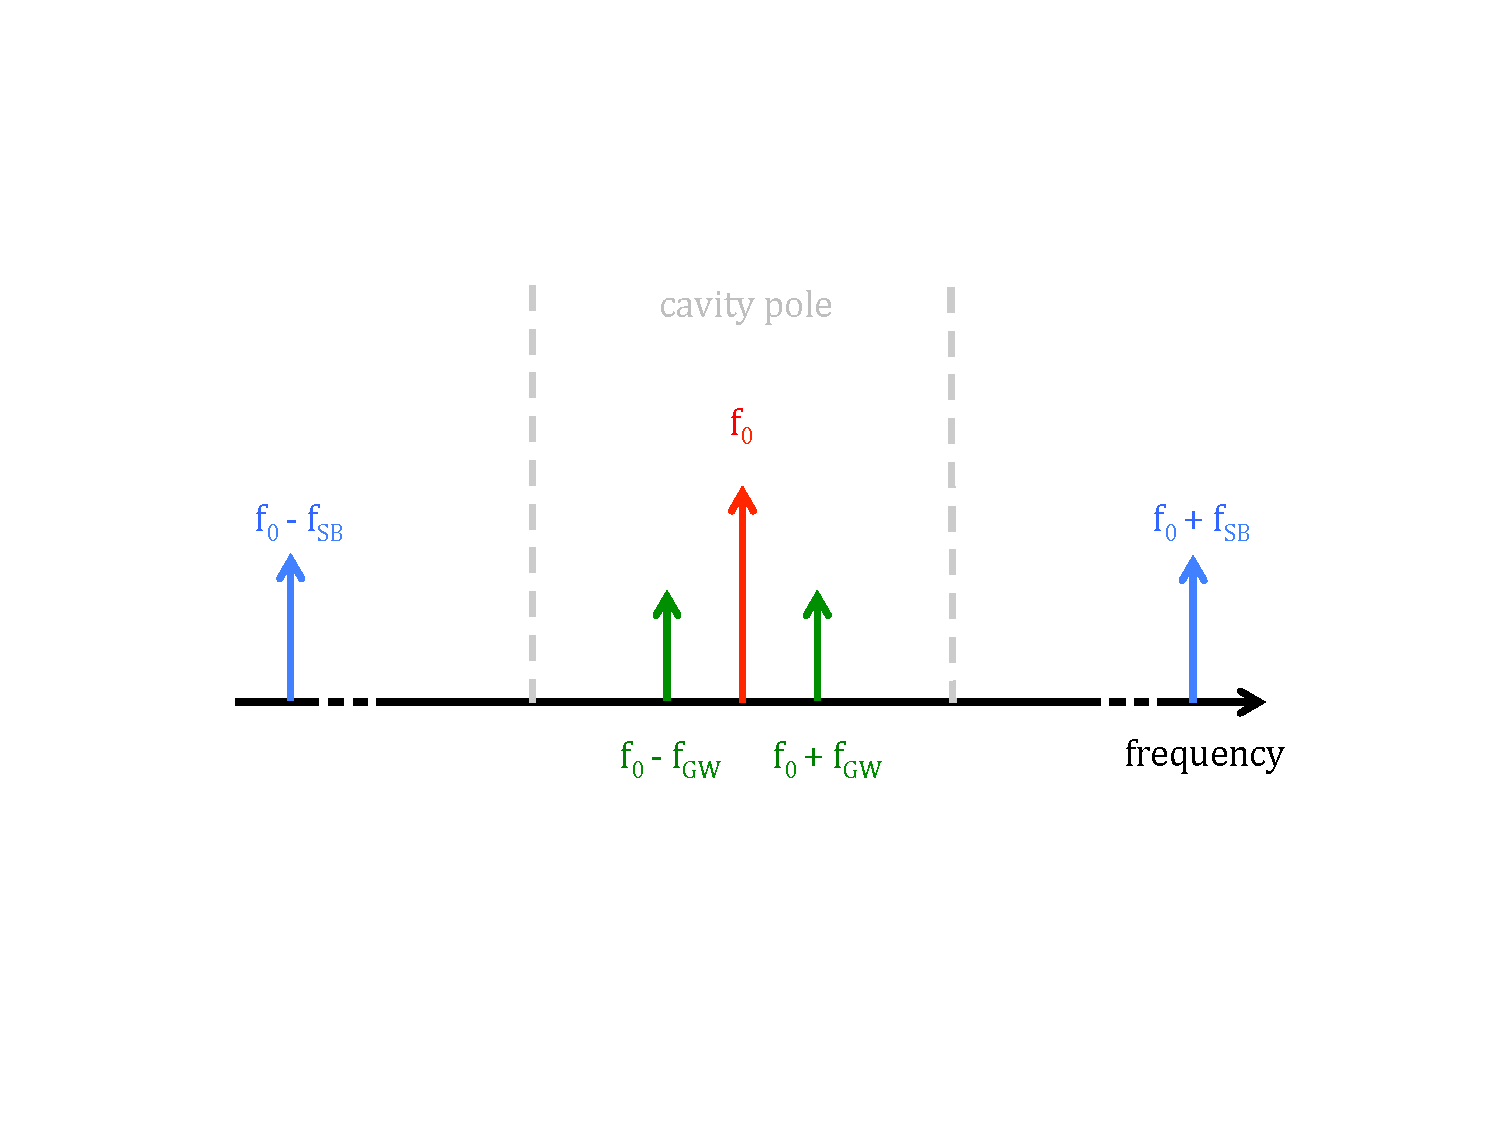
\includegraphics[width=\textwidth]{figures/introduction/omc-freq}
\caption[Sidebands and OMC cavity pole]{Frequency domain visualization of beam %
         at OMC. Grey dotted lines indicate the cavity pole. The gravitational %
         wave sidebands are within the cavity pole and are transmitted through %
         the OMC. The RF sidebands are in the MHz range and are rejected by the %
         OMC.}
\label{fig:omc-freq}
\end{figure}

\section{Sources of Gravitational Waves}

The data at the output of the interferometer must be carefully searched 
for evidence of gravitational wave signals. These signals have highly 
varying characteristics depending on the source of the gravitational 
waves. The gravitational wave strain produced depends on the distribution 
of energy at the source and is given as
\begin{equation}
h_{ij} = \frac{2}{r}\ddot{I}_{ij}
\end{equation}
where $\ddot{I}_{ij}$ is the quadropole tensor describing the 
energy distribution and $c=G=1$. This equation tells us that 
a source distribution requires an accelerating quadropole moment to 
generate gravitational waves. Depending on the dynamics of the source 
system, the resulting gravitational wave signals will vary greatly in 
both duration and morphology.

There are a number of potential sources of gravitational waves that are 
searched for in aLIGO data. Astrophysical searches include both modeled and unmodeled 
searches for both transient and continuous signals. Table \ref{tab:sources} 
gives an example of each of these sources.

\begin{table}[!ht]%
  \begin{tabular}{|c|c|c|}
  \hline
    & Transient  & Continuous  \\
  \hline
  Modeled & Compact binary coalescences & Targeted pulsars  \\
  \hline
  Unmodeled & Supernovae and GRBs  & Stochastic GW background \\
  \hline
  \end{tabular}
  \caption[Table of GW sources]{Table describing sources of %
           gravitational waves.}
  \label{tab:sources}
\end{table}

\subsection{Compact binary coalescences}

Compact binary coalescences (CBC) are the primary search target of the 
Advanced LIGO interferometers. These signals are the result of two 
compact objects, such as neutron stars or black holes, inspiraling 
in a decaying orbit until they merge and coalesce into one final 
compact object. The orbital frequency of such systems increases 
monotonically as the orbit decays, resulting in a gravitational 
wave signal that sweeps upwards in frequency known as a 'chirp'. 
Since the gravitational wave signal from such a system is known, 
this model is incorporated into the search algorithm and the 
search is referred to as a modeled search. CBC waveforms will 
have a duration from $\sim$0.1-60s in the frequency range that
aLIGO is sensitive to and as such they are considered transient 
signals. Searches for CBC 
signals are discussed in Section \ref{sec:cbc-search}.

Of particular interest to aLIGO are binary neutron star systems, 
which are known to exist from astronomical 
observation. The 1993 Nobel Prize in Physics was awared to Hulse and 
Taylor for the indirect detection of gravitational waves from a binary 
neutron star system. The orbital 
period of the Hulse-Taylor binary neutron star system has been measured 
since 1974. The decay of its orbital period matches the 
expected orbital decay based on energy loss due to the emission of 
gravitational waves. 

Beyond binary neutron stars, the search for compact binary coalescences 
is expanded to search for binary black hole (BBH) systems and neutron star-black 
hole (NSBH) systems. The discovery of gravitational waves from binary black holes 
was accomplished in the 
first observing run with the discovery of two binary black hole systems, GW150914 
and GW151226. Further discussion of the results from the first observing run is 
presented in Chapter \ref{ch:o1results}.

\subsection{Burst signals}

Transient 

\subsection{Continuous waves}


\subsection{Stochastic background}

Continuous waves from pulsars
Bursts from supernovae
Stochastic background


\section{Searching for Compact Binary Coalescences}\label{sec:cbc-search}

Steal this from O1 CBC DQ paper


\section{The Advanced Detector Network}

The Advanced Laser Interferometer Gravitational-Wave Observatory (aLIGO) is 
part of a worldwide effort to detect gravitational waves from astrophysical 
sources. The two aLIGO interferometers, one in Hanford, WA and one in 
Livingston, LA, are part of a growing network of ground-based interferometric 
gravitational wave detectors. Each aLIGO interferometer has 4km long arms 
arranged in an L-shaped configuration. A gravitational wave passing through 
an aLIGO interferometer will cause the arms to expand and contract, 
creating an interferometric signal at the output of the instrument. 
Section \ref{sec:aligo} contains a more detailed description of the aLIGO 
interferometers. 

There are a number of other interferometric gravitational wave detectors 
being built and commissioned for future use in collaboration with aLIGO.
The Advanced VIRGO detector is being built and commissioned in Cascina, Italy. 
When it is fully commissioned, VIRGO will be joining LIGO in observing runs. 
The VIRGO interferometer has 3km arms, which should provide enough 
sensitivity to allow for triangulation of astrophysical sources.

The GEO600 detector, located in Hanover, Germany is an interferometer built in 
collaboration between Germany and the United Kingdom. 
GEO600 is an extremely valuable test bed for interferometric technologies,
including quantum optics and homodyne detection. However, with 600m arms, GEO600 
is unlikely to be sensitive enough to witness expected astrophysical sources.

The KAGRA detector, located underground in the Kamioka mine in Japan, 
is in its commissioning phase. KAGRA has 3 km long arms and, 
unlike other gravitational wave interferometers, employs cryogenics to 
reduce thermal noise in its optics. When complete, KAGRA should be 
sensitive enough to contribute to the worldwide detector network.

Include that cool picture of the advanced detector network.
